%% psoc_api

API til styring af PSoC, herunder sensor og sprinkler, er implementeret i PSoC Creator. Top designet består af en ADC\_ SAR\_ Seq og to digitale pins til at styre henholdsvis sprinkler og Select til bestemmelse af temperatur- eller fugtighedsdata for SHT21P.
I top designet er der angivet følgende pins. ''ADC\_ in'', ''SLC'', ''sprinkler'' disse forbindes til henholdsvis pin P2[5], P0[0] og P2[0]. 

Under konfiguration for ADC-komponenten vælges Vref til VDDA og Single ended negative input vælges til Vss. Dette sætter ADCen op til at bruge 0 V som reference spænding.

Da PSoC kun har en SAR komponent er det nødvendigt at initialisere denne i sensorPackage-driveren.

\begin{figure}[htb]
\centering
{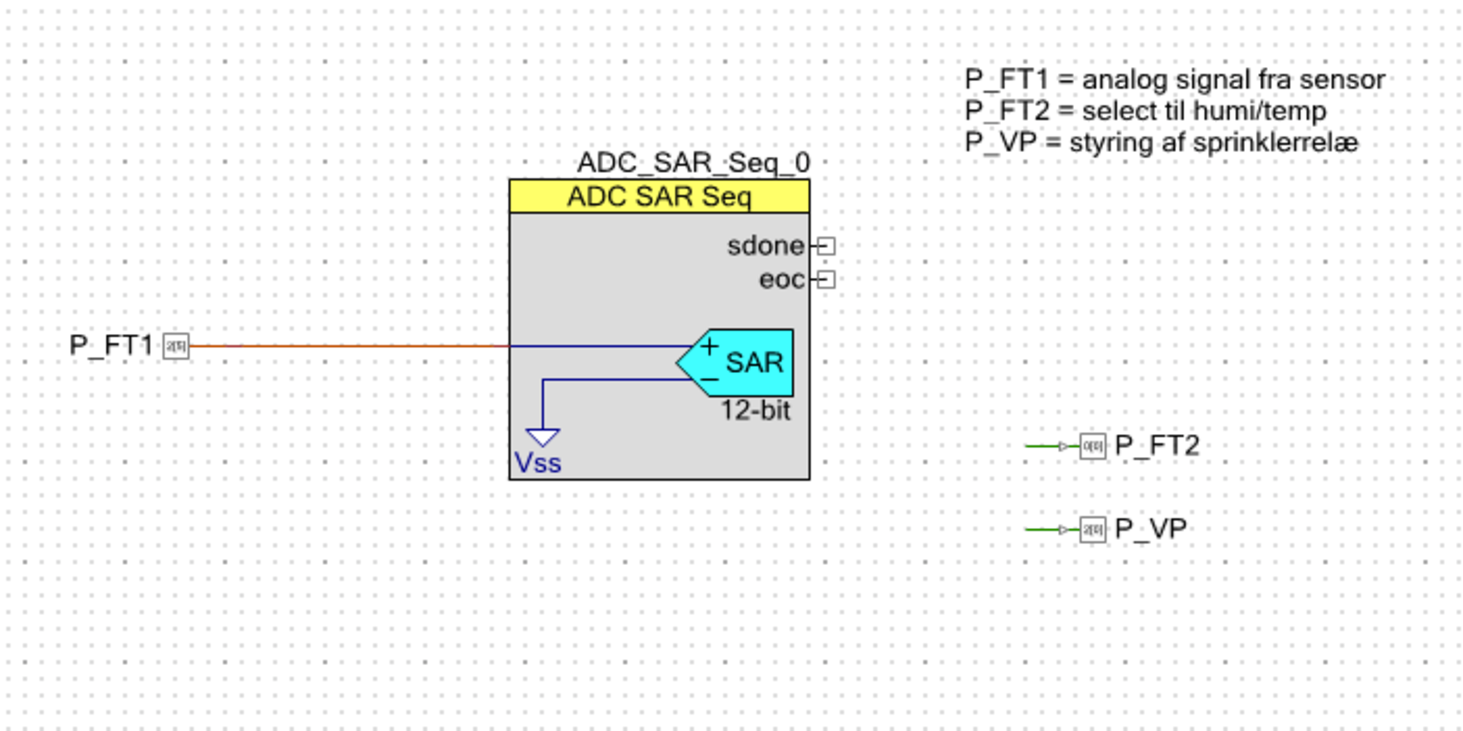
\includegraphics[width=0.60\textwidth]{filer/pics/psoc_api_topdesign.png}}
\caption{Top Design for PSoC API}
\label{lab:sht_filter}
\end{figure}

\begin{figure}[htb]
\centering
{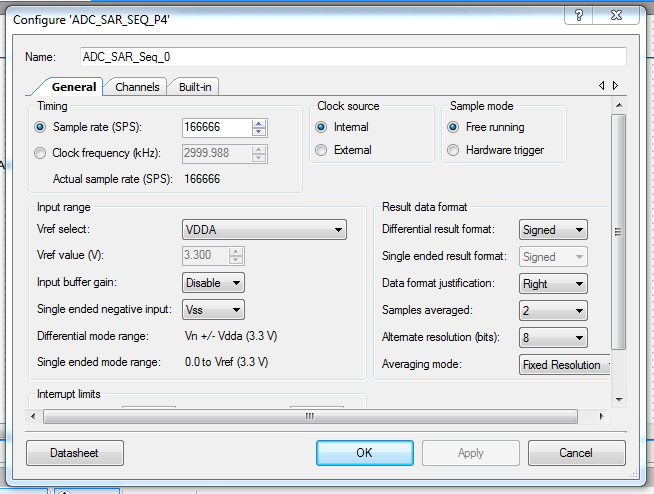
\includegraphics[width=0.60\textwidth]{filer/pics/psoc_api_config1.png}}
\caption{Konfiguration af Vref og Single ended negative input}
\label{lab:sht_filter}
\end{figure}

\begin{figure}[htb]
\centering
{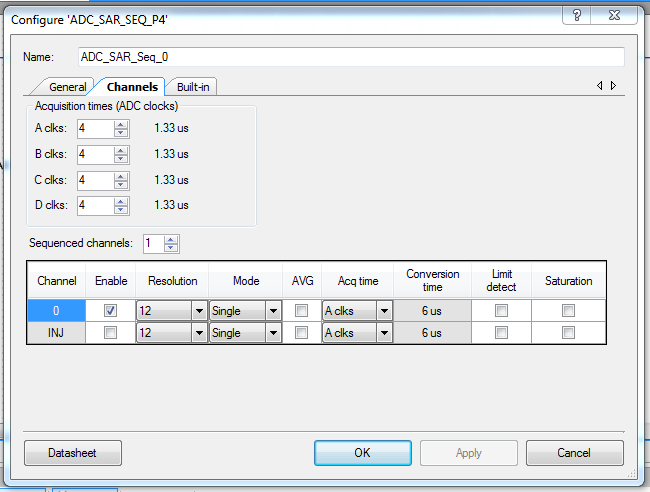
\includegraphics[width=0.60\textwidth]{filer/pics/psoc_api_config2.png}}
\caption{Konfiguration af Channels for PSoC API}
\label{lab:sht_filter}
\end{figure}